\subsection{Extension Requests}

\begin{frame}[c]{Project Lifecycle: Extension Requests}
    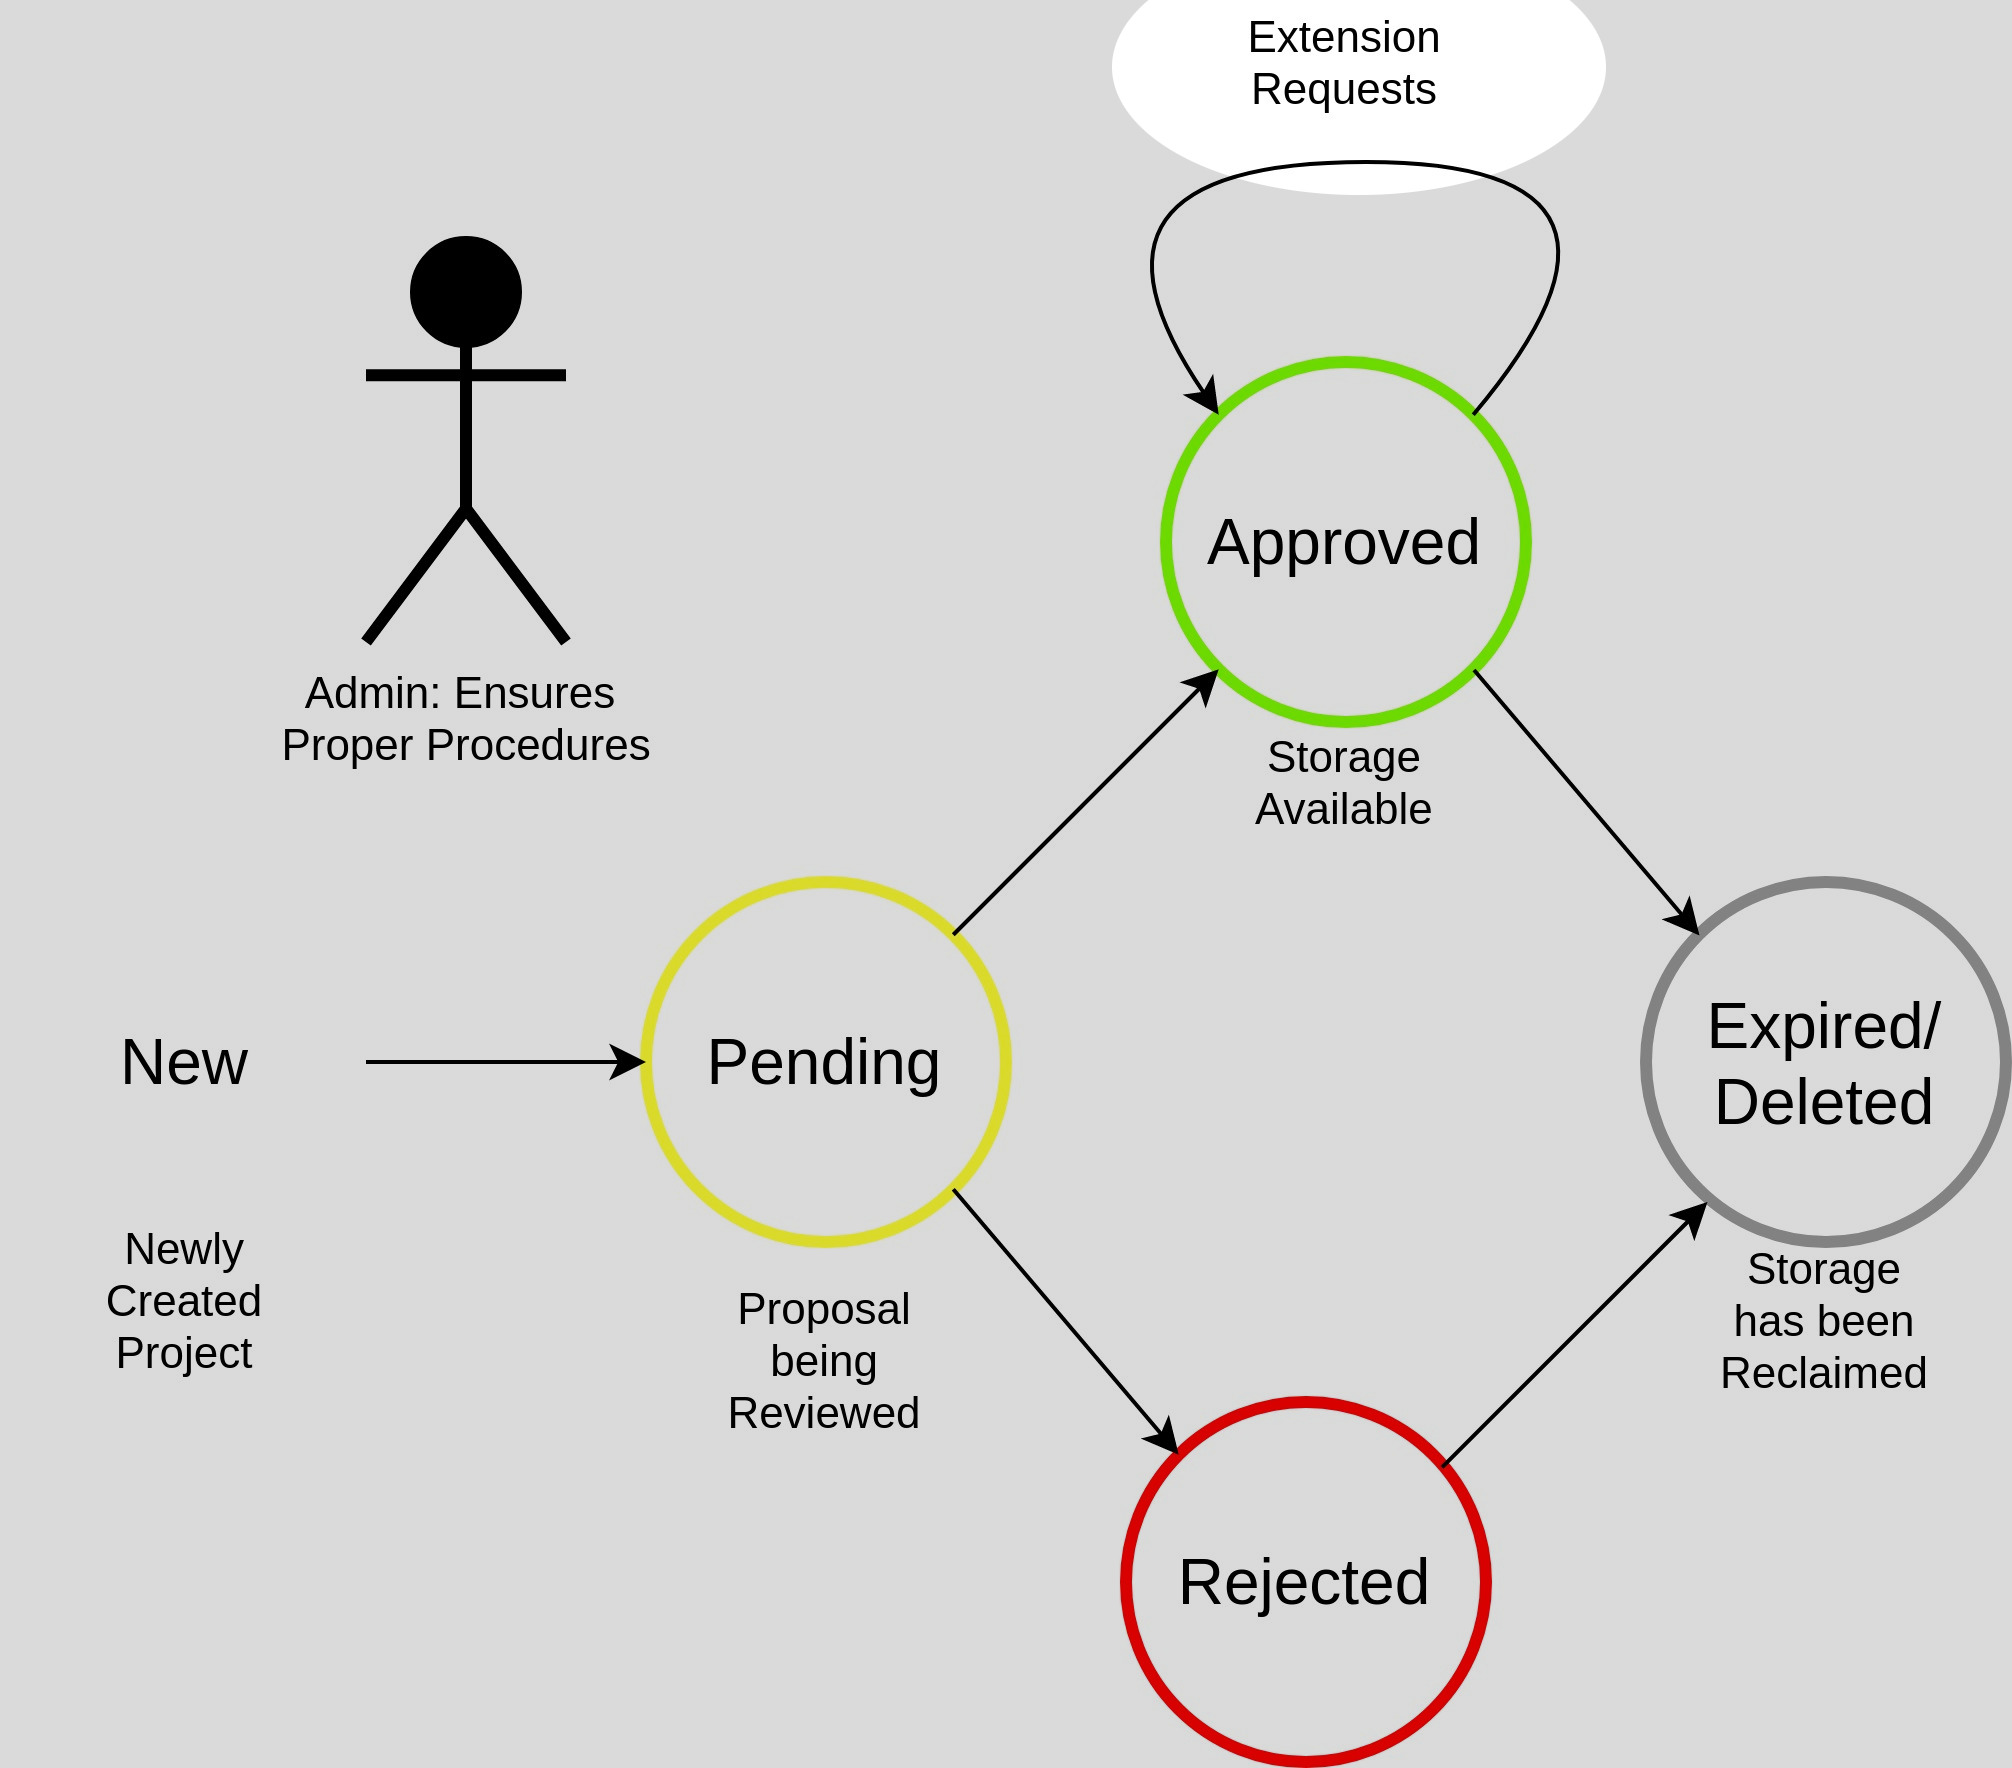
\includegraphics[height=0.9\textheight,center]{lsdf_states_requests}
\end{frame}

\begin{frame}[c]{Motivation}
    % It happens frequently that a project needs more space than initially
    % requested, or isn't done by the time their timeframe runs out (initial
    % timeframe was 4 Years). In these cases, timeframe and capacity can be
    % extended manually by an admin. To automate/improve this process, we
    % implemented it directly. Similar for capacity.
    % Verknüpfung mit zusätzliche Information abfragen!
    \begin{multicols}{2}
        Frequent Requests:
        \begin{itemize}[<+(1)->]
            \item More Storage
            \item Longer Timeframe
        \end{itemize}
        \pause
        Interaction with Admin not standardized:
        \begin{itemize}[<+(1)->]
            \item Mail
            \item Comments in Project
            \item ...
        \end{itemize}
        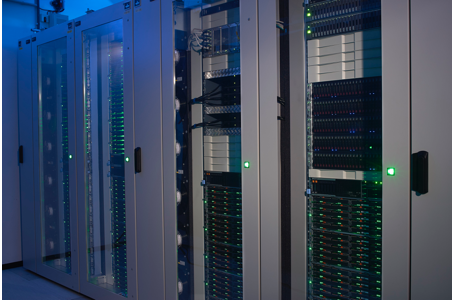
\includegraphics[width=0.5\textwidth]{storage1}
    \end{multicols}
\end{frame}


\pic{Timeframe Extension Request View}{19}
\pic{Capacity Extension Request View}{20}
\pic{Filled out Capacity Extension}{21}
\pic{Project: Extension System Message}{22}

\begin{frame}[c]{Routing for Timeframe Requests}
    \large
    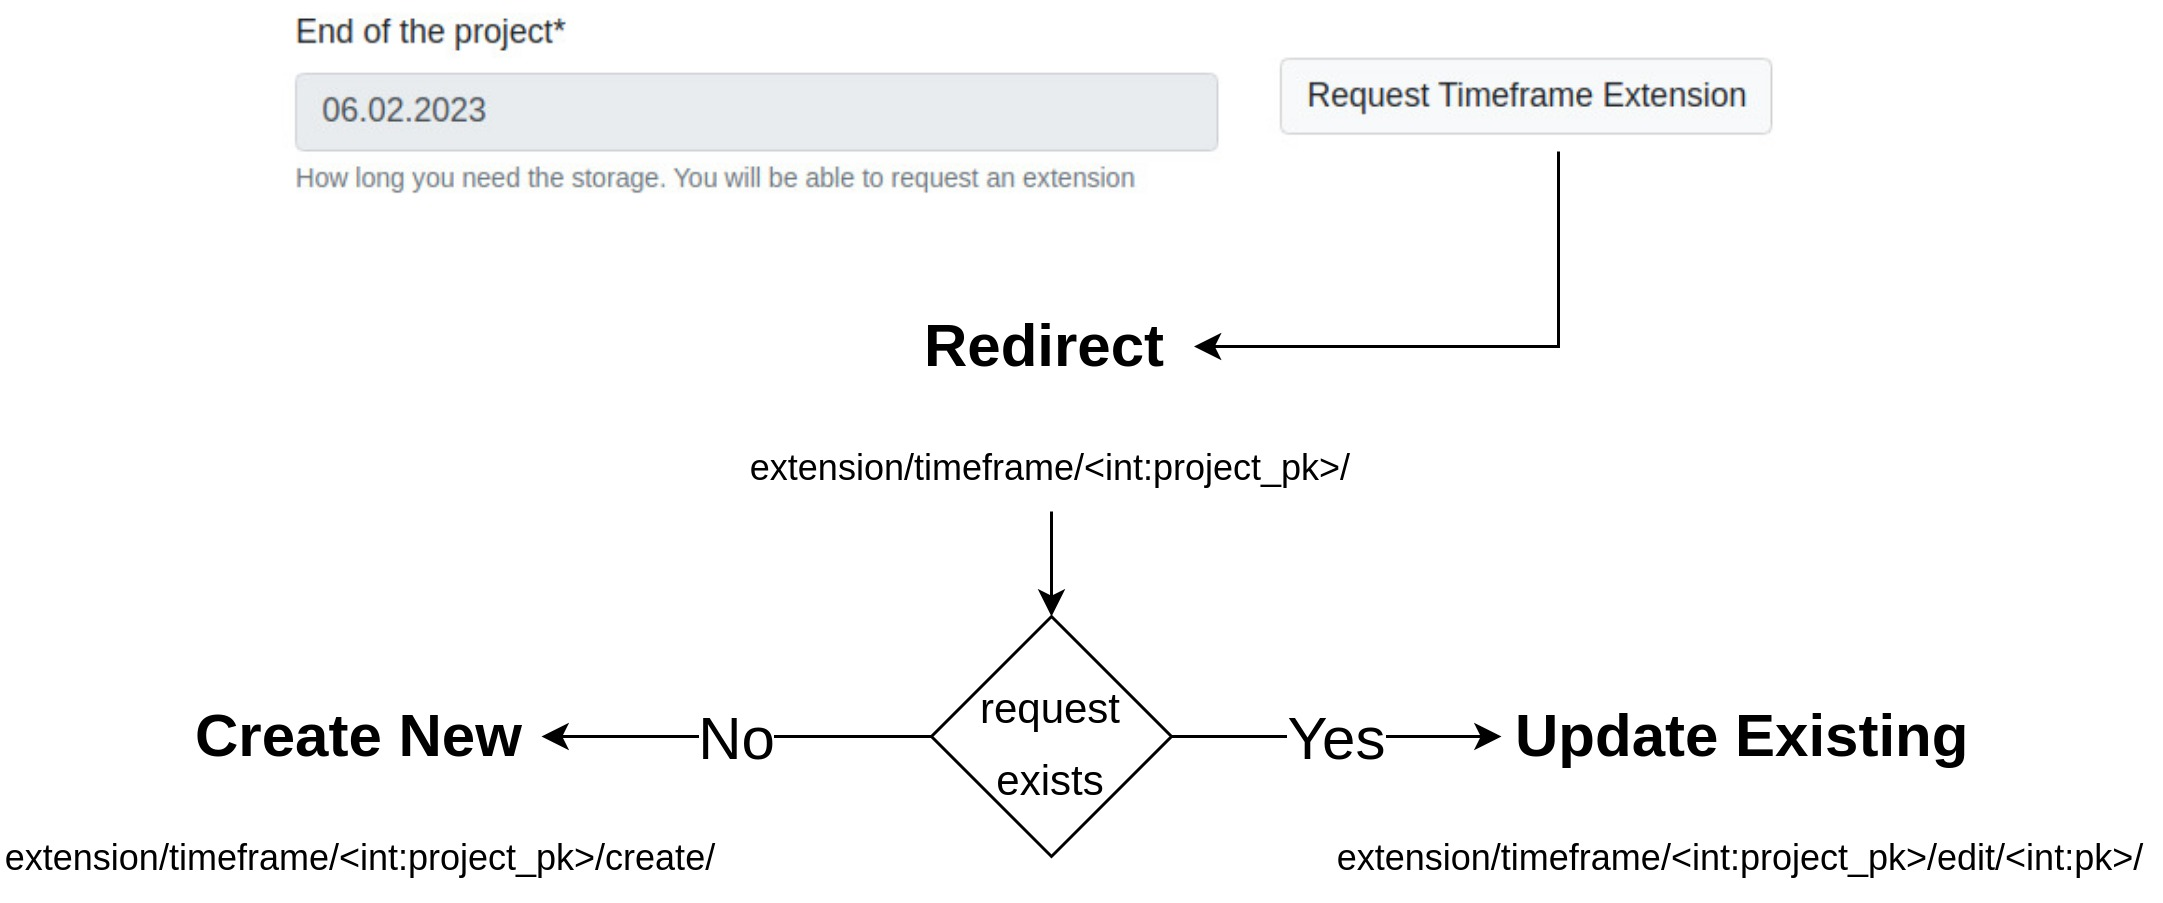
\includegraphics[width=\textwidth]{timeframe_routing}
\end{frame}

\pic{Admin: Extension Request Overview}{26}
\pic{System Message showing Extension Approval}{28}
\pic{Increased Capacity from User View}{29}

% \begin{frame}[c]{Extension Requests Admin View}
%     Include admin approval/reject
% \end{frame}
